\subsection{Stream Header}
The stream header \cref{tbl:header:stream}
contains all the necessary information
required to initialize the decoder.
In particular, it contains the pseudo-random
generator key that can be used to reproduce
the sparse binary sensing matrix used in the
encoder at the decoder,
the number of samples per window ($n$),
the number of measurements per window ($m$),
the number of ones per column in the sensing matrix
($d$),
and the maximum number of windows in each frame
of ECG signal ($w$).
It contains a flag indicating whether adaptive
or fixed quantization will be used.
It contains the limits on the normalized
root mean square error for
the adaptive quantization ($\rho$)
and adaptive clipping ($\gamma$) steps (elaborated subsequently).
If fixed quantization is used, then it contains
the fixed quantization parameter value ($q$).
Both $\rho$ and $\gamma$ in the stream header
are encoded using a simple decimal format $a \cdot 10^{-b}$ where $a$
and $b$ are encoded as 4-bit integers.

We then model the measurement values in $\hat{\by}$
as a quantized Gaussian distributed random variable
with mean $\mu_y$, standard deviation $\sigma_y$,
minimum value $\mu_y - r \sigma_y$ and maximum value $\mu_y + r \sigma_y$.

\subsubsection{Clipping}

An entropy coder can handle with a finite set of symbols
only. Hence, the range of input values [measurements
coded as integers] must be restricted to a finite range.
This is the reason one has to choose a distribution
with finite support (like quantized Gaussian).
From \cref{tbl:cs:codec:measure:stats} one can see that
while the complete range of measurement values can be
up to 40-50x larger than the standard deviation, the iqr
is less than $1.5$ times the standard deviation. In other
words, the measurement values are fairly concentrated
around its mean. This can be visually seen from the
histograms in \Cref{fig-cs-codec:y:hist:200} also.


\subsubsection{Measurement statistics}
Several aspects of our encoder architecture are based on the
statistics of the measurements $\by$. We collected the summary
statistics including mean $\mu$, standard deviation $\sigma$,
range of values in $\by$, skew and kurtosis
for the measurement values for each
of the ECG records in the MIT-BIH database. These values
have been reported for one particular encoder configuration
in \cref{tbl:cs:codec:measure:stats}.
In addition, we also compute the range divided by standard deviation
$\frac{\text{rng}}{\sigma}$
and the iqr (inter quantile range) divided by standard deviation
$\frac{\text{iqr}}{\sigma}$.


\subsection{Gaussianity}

Towards this, we measured the
skew and kurtosis for the measurements for each record
as shown in \cref{tbl:cs:codec:measure:stats}
for the sensing matrix configuration of $m=256,n=512,d=4$.
For a Gaussian distributed variable,
the skew should be close to $0$ while kurtosis should be close to $3$.
While the skew is not very high, Kurtosis does vary widely.

One can see that the divergence tends to increase as the
kurtosis increases. We determined the Pearson correlation
coefficient between kurtosis and kld to be $0.67$.


\Cref{fig-cs-codec:y:234:empirical:quantized} shows an example
where the empirical distribution is significantly different
from the corresponding quantized Gaussian distribution
due to the presence of a large
number of $0$ values in $\by$. Note that this is different
from the histograms in \cref{fig-cs-codec:y:hist:200} where
the $\by$ values have been binned into 200 bins.

\begin{figure}[htb]
    \centering % <-- added
  \centering 
  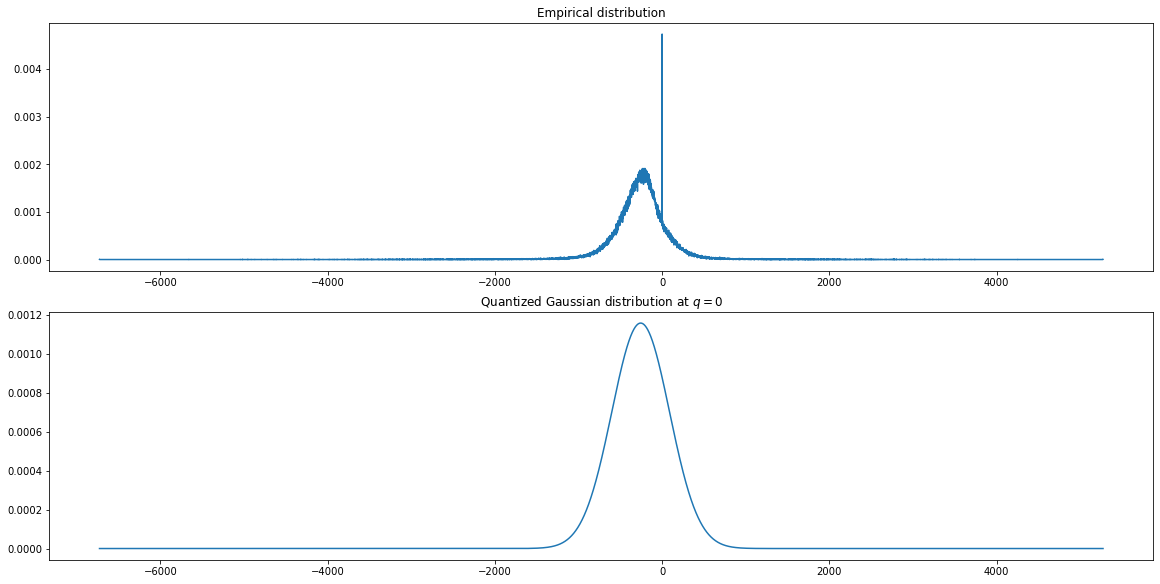
\includegraphics[width=0.95\linewidth]
  {images/rec_234_empirical_vs_quantized_gaussian.png}
\caption{Empirical and quantized Gaussian distributions for measurement values
$\by$ in record 234}
\label{fig-cs-codec:y:234:empirical:quantized}
\end{figure}

%%!TEX root = ../paper_ecg_cs_codec.tex
\begin{table}[ht]
\tiny
\centering
\caption{Measurement statistics at $m=256,n=512,d=4$}
\begin{tabular}{rrrrrrrrrr}
\toprule
 record &  $\mu_y$ &  $\sigma_y$ &  iqr &  rng &  skew &  kurtosis 
 & kld & $\frac{\text{rng}}{\sigma}$ &  $\frac{\text{iqr}}{\sigma}$ \\
\midrule
100 &  -490.0 &  224.4 &  293.0 &     2562 &    -0.5 &         3.7 & 0.049 &       11.4 &        1.3 \\
101 &  -454.8 &  287.1 &  323.0 &     9647 &    -0.4 &        15.4 &  0.13 &       33.6 &        1.1 \\
102 &  -393.4 &  197.0 &  257.2 &     2035 &    -0.6 &         3.7 & 0.053 &       10.3 &        1.3 \\
103 &  -370.3 &  285.9 &  302.0 &     8824 &    -0.8 &        15.9 &  0.16 &       30.9 &        1.1 \\
104 &  -360.1 &  231.5 &  284.0 &     4204 &    -0.6 &         5.0 & 0.071 &       18.2 &        1.2 \\
105 &  -360.2 &  346.7 &  326.0 &    13704 &    -0.4 &        22.5 &  0.24 &       39.5 &        0.9 \\
106 &  -284.7 &  270.6 &  314.0 &     4135 &    -0.1 &         4.4 & 0.046 &       15.3 &        1.2 \\
107 &  -372.2 &  624.6 &  747.0 &     9639 &    -0.5 &         4.6 & 0.062 &       15.4 &        1.2 \\
108 &  -365.9 &  422.3 &  336.0 &    12986 &    -0.2 &        22.1 &  0.36 &       30.7 &        0.8 \\
109 &  -368.5 &  335.5 &  389.0 &     7487 &     0.2 &         7.3 & 0.064 &       22.3 &        1.2 \\
111 &  -262.1 &  307.7 &  306.0 &    11998 &    -0.9 &        23.1 &   0.2 &       39.0 &        1.0 \\
112 & -1315.8 &  538.9 &  724.0 &     7839 &    -0.6 &         4.1 & 0.088 &       14.5 &        1.3 \\
113 &  -248.3 &  336.7 &  379.0 &     6121 &    -0.1 &         5.2 & 0.064 &       18.2 &        1.1 \\
114 &  -248.7 &  219.4 &  235.0 &     8756 &     1.2 &        30.4 &  0.14 &       39.9 &        1.1 \\
115 &  -780.8 &  461.1 &  559.0 &     9715 &    -0.8 &         6.7 & 0.094 &       21.1 &        1.2 \\
116 & -1498.1 &  874.9 &  930.0 &    35083 &    -0.3 &        22.7 &  0.22 &       40.1 &        1.1 \\
117 & -1363.0 &  560.1 &  748.0 &     9179 &    -0.7 &         4.4 & 0.098 &       16.4 &        1.3 \\
118 & -1373.1 &  613.9 &  809.0 &    10935 &    -0.5 &         4.4 &   0.1 &       17.8 &        1.3 \\
119 & -1378.1 &  629.0 &  825.0 &     8363 &    -0.6 &         3.8 & 0.074 &       13.3 &        1.3 \\
121 & -1295.5 &  635.2 &  763.0 &    17012 &    -1.4 &        13.1 &  0.16 &       26.8 &        1.2 \\
122 & -1349.7 &  555.2 &  747.0 &     7870 &    -0.6 &         3.7 & 0.079 &       14.2 &        1.3 \\
123 & -1274.2 &  514.1 &  699.0 &     6603 &    -0.6 &         3.8 & 0.084 &       12.8 &        1.4 \\
124 & -1293.1 &  678.9 &  829.0 &    11886 &    -0.6 &         5.4 &   0.1 &       17.5 &        1.2 \\
200 &  -168.8 &  261.8 &  288.0 &     6285 &    -0.3 &         7.7 &  0.08 &       24.0 &        1.1 \\
201 &  -255.9 &  189.5 &  196.0 &     9986 &     0.7 &        55.1 &  0.16 &       52.7 &        1.0 \\
202 &  -270.8 &  262.1 &  274.0 &    11421 &    -1.0 &        33.0 &  0.16 &       43.6 &        1.0 \\
203 &  -271.1 &  471.7 &  455.0 &    13371 &    -0.1 &        15.1 &   0.2 &       28.3 &        1.0 \\
205 &  -489.1 &  233.6 &  301.0 &     3257 &    -0.6 &         4.1 & 0.059 &       13.9 &        1.3 \\
207 &  -273.5 &  339.1 &  344.0 &    11400 &    -1.2 &        18.1 &  0.22 &       33.6 &        1.0 \\
208 &  -264.6 &  427.3 &  410.0 &    12449 &     0.4 &        16.5 &  0.18 &       29.1 &        1.0 \\
209 &  -263.6 &  249.6 &  292.0 &     4731 &    -0.5 &         4.9 & 0.065 &       19.0 &        1.2 \\
210 &  -250.9 &  228.3 &  249.0 &     7909 &     0.5 &        17.2 & 0.087 &       34.6 &        1.1 \\
212 &  -249.7 &  296.9 &  336.0 &     7232 &    -0.5 &         7.3 & 0.088 &       24.4 &        1.1 \\
213 &  -353.5 &  523.1 &  635.0 &     6528 &    -0.2 &         4.0 & 0.039 &       12.5 &        1.2 \\
214 &  -257.8 &  315.3 &  369.0 &     4248 &     0.2 &         4.1 &  0.04 &       13.5 &        1.2 \\
215 &  -243.0 &  208.7 &  256.0 &     3544 &    -0.3 &         4.2 & 0.039 &       17.0 &        1.2 \\
217 &  -264.2 &  458.7 &  528.0 &    11928 &    -0.3 &         8.5 & 0.089 &       26.0 &        1.2 \\
219 &  -938.8 &  687.6 &  811.0 &    10727 &    -0.4 &         4.6 & 0.074 &       15.6 &        1.2 \\
220 &  -864.8 &  378.5 &  503.0 &     4731 &    -0.5 &         3.7 & 0.059 &       12.5 &        1.3 \\
221 &  -262.4 &  228.0 &  270.0 &     3000 &    -0.1 &         4.1 & 0.036 &       13.2 &        1.2 \\
222 &  -250.4 &  212.1 &  252.0 &     4327 &    -0.8 &         5.7 & 0.085 &       20.4 &        1.2 \\
223 &  -818.4 &  419.1 &  529.0 &     7449 &    -0.6 &         5.0 & 0.068 &       17.8 &        1.3 \\
228 &  -221.5 &  356.9 &  294.0 &    11962 &    -1.0 &        24.0 &  0.35 &       33.5 &        0.8 \\
230 &  -271.8 &  285.3 &  308.0 &     7044 &    -0.4 &         8.6 &   0.1 &       24.7 &        1.1 \\
231 &  -253.1 &  228.9 &  278.0 &     3250 &    -0.3 &         4.2 & 0.042 &       14.2 &        1.2 \\
232 &  -242.2 &  191.9 &  243.0 &     2951 &    -0.4 &         4.0 & 0.039 &       15.4 &        1.3 \\
233 &  -245.9 &  427.2 &  480.0 &     9636 &    -0.1 &         6.5 & 0.083 &       22.6 &        1.1 \\
234 &  -257.2 &  345.1 &  316.0 &    12002 &    -0.7 &        19.8 &  0.25 &       34.8 &        0.9 \\
\bottomrule
\end{tabular}
\label{tbl:cs:codec:measure:stats}
\end{table}

%\begin{table}[ht]
\tiny
\centering
\caption{Compression statistics at $m=256,n=512,d=4$}
\begin{tabular}{rrrrrrrrrr}
\toprule
 record &  CR &  PSS &  bpm &  bps &  OH &  Q\_SNR &  SNR &  PRD &    QS \\
\midrule
    100 & 3.3 & 69.3 &  6.7 &  3.4 & 0.2 &   36.1 & 25.9 &  5.1 &  64.2 \\
    101 & 3.1 & 68.2 &  7.0 &  3.5 & 0.2 &   37.0 & 25.9 &  5.0 &  62.4 \\
    102 & 3.2 & 68.6 &  6.9 &  3.5 & 0.2 &   35.9 & 24.4 &  6.0 &  52.8 \\
    103 & 3.0 & 66.7 &  7.3 &  3.7 & 0.2 &   38.2 & 26.1 &  5.0 &  60.5 \\
    104 & 3.0 & 67.0 &  7.3 &  3.6 & 0.2 &   36.9 & 20.4 &  9.6 &  31.6 \\
    105 & 3.0 & 66.3 &  7.4 &  3.7 & 0.2 &   36.5 & 24.8 &  5.8 &  51.5 \\
    106 & 2.8 & 64.7 &  7.8 &  3.9 & 0.2 &   37.8 & 24.4 &  6.0 &  47.1 \\
    107 & 2.7 & 62.5 &  8.3 &  4.1 & 0.2 &   38.5 & 26.8 &  4.6 &  58.2 \\
    108 & 2.9 & 66.0 &  7.5 &  3.7 & 0.2 &   37.6 & 24.4 &  6.0 &  48.8 \\
    109 & 3.0 & 66.3 &  7.4 &  3.7 & 0.2 &   37.5 & 27.3 &  4.3 &  68.6 \\
    111 & 2.8 & 64.9 &  7.7 &  3.9 & 0.2 &   38.3 & 24.6 &  5.9 &  48.0 \\
    112 & 3.2 & 68.3 &  7.0 &  3.5 & 0.2 &   35.9 & 28.7 &  3.7 &  85.6 \\
    113 & 2.8 & 63.9 &  7.9 &  4.0 & 0.2 &   38.0 & 26.0 &  5.0 &  55.0 \\
    114 & 3.0 & 66.2 &  7.4 &  3.7 & 0.2 &   37.6 & 22.5 &  7.5 &  39.6 \\
    115 & 3.1 & 67.4 &  7.2 &  3.6 & 0.2 &   36.3 & 27.5 &  4.2 &  72.6 \\
    116 & 3.0 & 66.5 &  7.4 &  3.7 & 0.2 &   36.2 & 27.6 &  4.2 &  71.6 \\
    117 & 3.2 & 68.3 &  7.0 &  3.5 & 0.2 &   35.6 & 28.8 &  3.6 &  87.0 \\
    118 & 3.1 & 67.4 &  7.2 &  3.6 & 0.2 &   38.3 & 27.1 &  4.4 &  69.4 \\
    119 & 3.0 & 67.1 &  7.2 &  3.6 & 0.2 &   37.5 & 29.0 &  3.6 &  85.6 \\
    121 & 3.1 & 67.6 &  7.1 &  3.6 & 0.2 &   37.1 & 30.7 &  2.9 & 106.5 \\
    122 & 3.1 & 68.0 &  7.0 &  3.5 & 0.2 &   35.6 & 27.9 &  4.0 &  78.0 \\
    123 & 3.2 & 68.6 &  6.9 &  3.5 & 0.2 &   35.6 & 28.3 &  3.8 &  82.8 \\
    124 & 3.0 & 67.2 &  7.2 &  3.6 & 0.2 &   37.3 & 30.0 &  3.2 &  96.7 \\
    200 & 2.8 & 63.7 &  8.0 &  4.0 & 0.2 &   37.5 & 22.2 &  7.8 &  35.3 \\
    201 & 3.0 & 67.0 &  7.3 &  3.6 & 0.2 &   38.1 & 26.2 &  4.9 &  61.8 \\
    202 & 2.9 & 65.1 &  7.7 &  3.8 & 0.2 &   38.4 & 25.8 &  5.1 &  55.9 \\
    203 & 2.8 & 64.0 &  7.9 &  4.0 & 0.2 &   38.2 & 22.7 &  7.3 &  38.0 \\
    205 & 3.2 & 69.1 &  6.8 &  3.4 & 0.2 &   36.2 & 25.8 &  5.1 &  62.9 \\
    207 & 2.8 & 64.6 &  7.8 &  3.9 & 0.2 &   37.4 & 25.5 &  5.3 &  53.4 \\
    208 & 2.8 & 63.9 &  8.0 &  4.0 & 0.2 &   37.9 & 24.7 &  5.8 &  47.7 \\
    209 & 2.8 & 64.5 &  7.8 &  3.9 & 0.2 &   38.4 & 20.3 &  9.7 &  29.0 \\
    210 & 2.9 & 65.3 &  7.6 &  3.8 & 0.2 &   38.3 & 24.4 &  6.1 &  47.7 \\
    212 & 2.8 & 64.3 &  7.9 &  3.9 & 0.2 &   37.8 & 20.1 &  9.9 &  28.2 \\
    213 & 2.7 & 63.6 &  8.0 &  4.0 & 0.2 &   38.6 & 22.7 &  7.3 &  37.6 \\
    214 & 2.8 & 64.0 &  7.9 &  4.0 & 0.2 &   37.6 & 26.7 &  4.6 &  60.0 \\
    215 & 2.9 & 65.3 &  7.6 &  3.8 & 0.2 &   37.5 & 19.8 & 10.2 &  28.2 \\
    217 & 2.8 & 64.3 &  7.8 &  3.9 & 0.2 &   37.1 & 27.0 &  4.5 &  62.5 \\
    219 & 3.0 & 66.7 &  7.3 &  3.7 & 0.2 &   36.9 & 29.0 &  3.6 &  84.4 \\
    220 & 3.3 & 69.6 &  6.7 &  3.3 & 0.2 &   35.1 & 26.6 &  4.7 &  69.9 \\
    221 & 2.9 & 65.1 &  7.7 &  3.8 & 0.2 &   38.9 & 24.9 &  5.7 &  50.5 \\
    222 & 2.9 & 65.6 &  7.6 &  3.8 & 0.2 &   37.6 & 22.0 &  7.9 &  36.8 \\
    223 & 3.1 & 68.0 &  7.0 &  3.5 & 0.2 &   36.3 & 27.9 &  4.0 &  77.8 \\
    228 & 2.8 & 64.5 &  7.8 &  3.9 & 0.2 &   36.9 & 22.9 &  7.1 &  39.4 \\
    230 & 2.8 & 64.6 &  7.8 &  3.9 & 0.2 &   38.2 & 24.7 &  5.9 &  48.2 \\
    231 & 2.9 & 65.6 &  7.6 &  3.8 & 0.2 &   38.2 & 25.5 &  5.3 &  54.8 \\
    232 & 3.0 & 66.8 &  7.3 &  3.7 & 0.2 &   37.9 & 22.8 &  7.3 &  41.4 \\
    233 & 2.8 & 63.8 &  8.0 &  4.0 & 0.2 &   37.9 & 24.9 &  5.7 &  48.8 \\
    234 & 2.8 & 64.6 &  7.8 &  3.9 & 0.2 &   37.3 & 25.2 &  5.5 &  51.6 \\
\bottomrule
\end{tabular}
\label{tbl:comp:stats:m=256:n=512:d=4}
\end{table}

\begin{table}[ht]
\tiny
\centering
\caption{Summary compression statistics at $m=256,n=512,d=4$}
\begin{tabular}{lrrrrrrrrr}
\toprule
{} &  CR &  PSS &  bpm &  bps &  OH &  Q\_SNR &  SNR &  PRD &    QS \\
\midrule
mean & 3.0 & 66.0 &  7.5 &  3.7 & 0.2 &   37.3 & 25.4 &  5.6 &  57.8 \\
std  & 0.2 &  1.8 &  0.4 &  0.2 & 0.0 &    0.9 &  2.6 &  1.8 &  18.6 \\
min  & 2.7 & 62.5 &  6.7 &  3.3 & 0.2 &   35.1 & 19.8 &  2.9 &  28.2 \\
50\%  & 2.9 & 66.1 &  7.5 &  3.7 & 0.2 &   37.5 & 25.7 &  5.2 &  54.9 \\
max  & 3.3 & 69.6 &  8.3 &  4.1 & 0.2 &   38.9 & 30.7 & 10.2 & 106.5 \\
\bottomrule
\end{tabular}
\label{tbl:comp:summary:m=256:n=512:d=4}
\end{table}

Note that often in literature, $\pss$ is defined as compression ratio
(e.g., \cite{mamaghanian2011compressed}).
Several papers ignore the bitstream formation aspect
and report $\frac{m}{n} \times 100$
(e.g., \cite{zhang2016comparison})
or $\frac{n - m}{n} \times 100$ (e.g., \cite{zhang2021csnet})
as the compression ratio
which measures the reduction in number of measurements
compared to the number of samples in each window.

The measurement ratio $\frac{m}{n}$ is not a
good indicator of compression ratio.
If the sensing matrix $\Phi$ is Gaussian,
then the measurement values are real valued.
In literature using Gaussian sensing matrices
(e.g., \cite{zhang2016comparison}),
it is unclear how many bits are
being used to represent each floating point measurement value
for transmission.
Under standard 32-bit IEEE floating point format,
each value would require 32-bits.
Then for MIT-BIH data the compression ratio in bits
would be $\frac{11 \times n}{32 \times m}$.
The only way the ratio $\frac{m}{n}$ would make sense
if the measurements are also quantized at 11 bits
resolution. However the impact of such quantization
is not considered in the simulations.

Now consider the case of a sparse binary sensing
matrix. Since it consists of only zeros and ones,
hence for integer inputs, it generates integer
outputs. Thus, we can say that output of a sparse
binary sensor are quantized by design.
However, the range of values changes.
Assume that the sensing matrix has $d$ ones per column.
Then it has a total of $n d$ ones. Thus, each row
will have on average $\frac{n d}{m}$ ones.
\footnote{Since the ones are randomly placed, hence
we won't have same number of ones in each row.}
If we assume the input data to be in the range
of $[-1024, 1023]$ (under 11-bit), then in the
worst case, the range of output values may go
up to$[-\frac{n d}{m} \times 1024, \frac{n d}{m} \times 1023]$.
For a simple case where $n = 2m$ and $d=4$, we will require
14 bits to represent each measurement value.
To achieve $\frac{m}{n}$ as the compression ratio, we will
have to quantize the measurements in 11 bits. If we do so,
we shall need to provide some way to communicate the quantization
parameters to the decoder as well as study the impact of
quantization noise.
This issue seems to be ignored in \cite{zhang2012compressed}.


Since the entropy coder is coding the measurements rather than
the samples directly, hence it is also useful to see how
many bits are needed to code each measurement. We
denote this

As one desires higher compression ratios and lower
$\prd$, one can define a combined \emph{quality score} (QS) as
\begin{equation}
\text{QS} = \frac{\compr}{\prd} \times 100.
\end{equation}
\subsection{Performance Metrics}
\label{sec:codec:metrics}
In our encoder, digital ECG signal is split into windows
of $n$ samples each which can be multiplied
with a sensing matrix. 


\section{Intro}
Noncommunicable diseases (NCDs) account for 72\%
of all global deaths with cardiovascular diseases
(CVDs) accounting for 44\% of all NCD mortality
\cite{collins2019interact}.
For patients with CVDs, wearable device based remote ECG
monitoring plays a critical role in their disease
management and care. 


However, long term ECG monitoring
can generate a large amount of uncompressed data.
For example, each half hour 2 lead recording in the
MIT-BIH Arrhythmia database \cite{moody2001impact}
requires 1.9MB of storage. As shown in \cite{mamaghanian2011compressed},
in a real time telemonitoring sensor node, the wireless
transmission of data consumes most of the energy.
The real time compression of ECG data by a low
complexity encoder has received significant attention
in the past decade.

ECG signal compression has been an active area
of interest for several decades. Extensive surveys
can be found in \cite{singh2015review,rajankar2019electrocardiogram}.
Compressive sensing (CS) based techniques for ECG
data compression have been reviewed in 

Transform domain techniques
(e.g., Discrete Cosine Transform \cite{al1995dynamic},
Discrete Cosine Transform \cite{batista2001compression,bendifallah2011improved},
Discrete Wavelet Transform \cite{djohan1995ecg,lu2000wavelet,pooyan2004wavelet,kim2006wavelet}) are popular in ECG compression
and achieve high compression ratios (CR) at clinically
acceptable quality.
However, these are computationally intensive sparsifying
transforms on all data samples and are thus not suitable
for WBAN sensor nodes \cite{craven2014compressed}.

In order to keep the sensing matrix multiplication
simple and efficient, sparse binary sensing matrices
are a popular choice \cite{mamaghanian2011compressed,zhang2012compressed}.

We consider whether a digital quantization of the compressive
measurements affects the reconstruction quality.
Further, we study the empirical distribution of compressive
measurements to explore efficient ways of entropy coding
of the quantized measurements.

so that it
can be implemented efficiently in low-power devices


However, they don't
provide much detail on how the codebook was designed or how should
it be adapted for variations in ECG signals.
They clearly define the compression ratio in terms
of a ratio between the uncompressed bits $\bits_u$
and the compressed bits $\bits_c$. They define it
as $\frac{\bits_u - \bits_c}{\bits_u} \times 100$.
This is often known in literature as
\emph{percentage space savings}.

\Cref{appsec:cs} provides a short overview on
compressive sensing.
\Cref{appsec:ec} provides a short overview on
entropy coding.

Zhang et al. \cite{zhang2012compressed},
Zhang et al. \cite{zhang2021csnet} define
$\frac{n - m}{n} \times 100$ as compression ratio. 
Mangia et al. \cite{mangia2020deep} define $\frac{n}{m}$
as the compression ratio.
Polania et al. \cite{polania2018compressed} define
$\frac{m}{n}$ as compression ratio.
Picariello et al. \cite{picariello2021novel} use
a non-random sensing matrix.
They infer a circulant binary sensing matrix
directly from the ECG signal being compressed.
The sensing matrix is adapted as and when
there is significant change in the signal
statistics.
They represent both the ECG samples and
compressive measurements with same number of
bits per sample/measurement. However,
in their case, there is the additional
overhead of sending the sensing matrix updates.
Their compression ratio is slightly lower than
$\frac{n}{m}$ where they call $\frac{n}{m}$ as
the \emph{under-sampling ratio}.

Luo et al. in \cite{luo2014dynamic} proposed a dynamic
compression scheme for ECG signals which consisted
of a digital integrate and fire sampler followed
by an entropy coder. They used Huffman codes for
entropy coding of the timestamps associated with
the impulse train.

Chouakri et al. in \cite{chouakri2013wavelet} compute
the DWT of ECG signal by Db6 wavelet, select coefficients
using higher order statistics thresholding, then perform
linear prediction coding and Huffman coding of the selected
coefficients.  

\emph{zstd} by Facebook Inc. \cite{zstd}
and \emph{LZFSE} by Apple Inc. are popular lossless
data compression formats based on ANS.
